\section{Materials \& Methods}

Here, we propose an comparative method for co-diversifying systems that extends an approach developed by Lewitus and Morlon \cite{lewitus2015characterizing} for use with phylogenetic trees. The graph adjacency matrixes for each phylogenetic tree are constructed, as per Lewitus and Morlon. The total phylogenetic distance for each tree is then normalized to unity. Then, the adjacency matrixes for the two trees are joined along a common diagonal, creating two empty rectangular blocks symmetric about the diagonal. These rectangular blocks are where the any between the two joined graphs must exist, and so the interactions between the leaf nodes in the phylogeny are placed here, weighted at the mean branch length of the two trees. The graph Laplacian is constructed (Figure \ref{fig:FP_ajlp}), the eigenvalues are computed and a spectral density distribution (Figure \ref{fig:FP_eigendensity}) is computed using a kernel density estimator with a Gaussian kernel, as in Lewitus and Morlon. 

\subfile{FishPoo/figures/figure8}

The eigenvalues of a network's Laplacian corresponds to the frequency with which a random walker would visit each node in steady state (i.e., in the limit of the number of random steps as the number of steps approaches infinity). In a network with edge weights (or a tree with branch lengths), the probability distribution of random steps made by the walker from each node is partitioned by the edge weights (or branch lengths) of each edge connected connected to that node. It is a measure of the relative connectivity of each node in the network. 

\subfile{FishPoo/figures/figure9}

The eigenvalues of a network comprise its spectrum. A network's spectrum is a not perfectly unique; very small networks with different topologies may share the same eigenvalues. The probability of one tree being a superset of another approaches unity in the limit of very large trees. For trees of intermediate size ($ \approx 5 < n < n \rightarrow \infty$), the probability that two randomly selected trees will share the same spectrum is finite but negligible. \cite{matsen2012ubiquity} For networks constructed from two interconnected trees, individual internal nodes of the trees will have the same connectivity regardless of whether they are in a network or in a tree. Thus, the spectrum of such a network will be composed of eigenvalues that correspond to those of the internal nodes of each of the two trees, and a third group of eigenvalues corresponding to the leafs and their interactions. There are more possible configurations for networks of this general topology than for trees of a given number of nodes, and thus a larger number of spectra are possible for a network than for a tree.

Spectra are a discrete set of values equal to the number of nodes in the network, and so comparing the structure of networks with unequal sizes requires some additional transformation. As with Lewitus and Morlon, and Matsen and Evans \cite{lewitus2015characterizing, matsen2012ubiquity} work with trees, we map the Laplacian spectra into a continuous, unit space by applying a Gaussian kernel density estimator, yielding a continuous distribution function for each spectra. The dissimilarity between two distribution can be measured using the Kullback-Leibler divergence, $D_{\rm KL}$. 

\begin{equation}
    D_{\rm KL}( p, q ) = \int_{-\infty}^\infty p(x) \, \log\frac{p(x)}{q(x)} \, {\rm d}x
\end{equation}

\noindent The Kullback-Leibler divergence measures the information lost when using distribution $q(x)$ to approximate distribution $p(x)$. This is almost what we want, but unfortunately $D_{\rm KL}$, like subtraction and division, is not metric (in general, $D_{\rm KL}(p,q) \neq D_{\rm KL}(q,p)$ unless $p=q$, in which case $D_{\rm KL}=0$). However, the Jensen-Shannon divergence between the two distributions is metric.

\begin{equation}
    D_{\rm SJ}( p, q ) = \sqrt{ \frac{1}{2} D_{\rm KL}( p, q ) + \frac{1}{2} D_{\rm KL}( q, p ) }
\end{equation}

\noindent To demonstrate how this metric performs, we compare permutations of the Gopher/Louse dataset from Hafner {\em et al.}. Keeping the tree structures intact, a collection of spectra were computed by randomly reassigning links between leaf nodes (Figure \ref{fig:FP_ajperm}) and computing the Jensen-Shannon divergence between successively more permuted spectral distributions and the spectral distribution of the original, un-permuted graph (Figure \ref{fig:FP_permuted_distances}). The metric is neither linear nor monotonic with these permutations, but it does diverge predictably. 

\subfile{FishPoo/figures/figure10}

\subfile{FishPoo/figures/figure11}

\subfile{FishPoo/figures/figure12}

In this way, a feature space constructed over the Laplacian spectra of networks of interaction species with known ecologies (parasitic verses mutualistic interactions, for example). These networks are then projected into the space which they span, and a classifier is trained on their ecological labels. The spectra of interactions with unknown ecological labels are then projected into that space, and the trained classifier may then predict which ecological label is most likely for each unlabeled interaction.

For each interaction collected from the literature (which we'll denote $G_{L,i}$, there is a label for the type of ecological interaction taking place. Each spectral density distribution has a set of endogenous features (see also Table \ref{FP_studies_table}) :

\begin{itemize}
    \item{\textbf{Links} ($n_{L}$)} The number of links connecting the interacting trees.

    \item{\textbf{Occupancy} ($k$)} The ratio of the number of links to the number of leafs ($2 n_{L} : n_{\rm hosts} + n_{\rm guests}$).

    \item{\textbf{Squareness} ($q$)} : The ratio of the number of leafs in each tree.

    \item{\textbf{Eigengap} ($\lambda_{\delta}$)} The difference between the largest and second largest eigenvalues in the Laplacian spectrum.
    
    \item{\textbf{Kurtosis} ($\gamma_{2}$)} The sharpness of the peak in the distribution (the fourth standardized moment).

    \item{\textbf{Skew} ($\gamma_{1}$)} The asymmetry of the distribution (the third standardized moment).

    \item{\textbf{Hommola correlation} ($r_{H}$)} The Hommola correlation of the interaction \cite{hommola2009permutation}.

    \item{\textbf{Hommola significance} ($p_{H}$)} The significance of the Hommola correlation \cite{hommola2009permutation}.

    \item{\textbf{Tree distance} ($D_{t}$)} The Jensen-Shannon divergence between the spectral density distributions of each of the two phylogenetic trees in the interactions.
\end{itemize}

\noindent These properties form an $n\times 9$ matrix of features, like so :

\begin{equation}
\psi =
\bordermatrix{
        & \lambda_{\delta}   & \gamma_{1}   & \gamma_{2}   & r_{H}   & p_{H}   & D_{t}   & k      & q      & n_{L}   \cr
G_{L,0} & \lambda_{\delta,0} & \gamma_{1,0} & \gamma_{2,0} & r_{H,0} & p_{H,0} & D_{t,0} & k_{0}  & q_{0}  & n_{L,0} \cr
G_{L,1} & \lambda_{\delta,1} & \gamma_{1,1} & \gamma_{2,1} & r_{H,1} & p_{H,1} & D_{t,1} & k_{1}  & q_{1}  & n_{L,1} \cr
G_{L,2} & \lambda_{\delta,2} & \gamma_{1,2} & \gamma_{2,2} & r_{H,2} & p_{H,2} & D_{t,2} & k_{2}  & q_{2}  & n_{L,2} \cr
\vdots  & \vdots             & \vdots       & \vdots       & \vdots  & \vdots  & \vdots  & \vdots & \vdots & \vdots  \cr 
G_{L,n} & \lambda_{\delta,n} & \gamma_{1,n} & \gamma_{2,n} & r_{H,n} & p_{H,n} & D_{t,n} & k_{n}  & q_{n}  & n_{L,n} \cr
}
\end{equation}

\noindent There are also the Shannon-Jensen distances between each pair of labeled interactions :

\begin{equation}
    D_{L,L,i,j} = D_{\rm SJ}( G_{L,i}, G_{L,j} )
\end{equation}

\noindent These distances form an matrix of $n^2$ features, like so :

\begin{equation}
\xi_L =
\bordermatrix{
        & G_{L,0}     & G_{L,1}     & G_{L,2}     & \cdots & G_{L,n}     \cr
G_{L,0} & D_{L,L,0,0} & D_{L,L,0,1} & D_{L,L,0,2} & \cdots & D_{L,L,0,n} \cr
G_{L,1} & D_{L,L,1,0} & D_{L,L,1,1} & D_{L,L,1,2} & \cdots & D_{L,L,1,n} \cr
G_{L,2} & D_{L,L,2,0} & D_{L,L,2,1} & D_{L,L,2,2} & \cdots & D_{L,L,2,n} \cr
\vdots  & \vdots      & \vdots      & \vdots      & \ddots & \vdots      \cr
G_{L,n} & D_{L,L,n,0} & D_{L,L,n,1} & D_{L,L,n,2} & \cdots & D_{L,L,n,n} \cr
}
\end{equation}

\noindent Together, these two matrixes form the feature space into which we will use to define the system.

\begin{equation}
    \Psi_{L} = \left[ \psi_{L,(n \times 9)} | \xi_{L,(n \times n)} \right]
\end{equation}

Interactions with unknown ecology (unlabeled interactions) can then be placed into this space. Like the labeled interactions, the endogenous properties of the Laplacean spectra are tabulated :

\begin{equation}
\psi_U =
\bordermatrix{
        & \lambda_{\delta}   & \gamma_{1}   & \gamma_{2}   & r_{H}   & p_{H}   & D_{t}   & k      & q      & n_{L}   \cr
G_{U,0} & \lambda_{\delta,0} & \gamma_{1,0} & \gamma_{2,0} & r_{H,0} & p_{H,0} & D_{t,0} & k_{0}  & q_{0}  & n_{L,0} \cr
G_{U,1} & \lambda_{\delta,1} & \gamma_{1,1} & \gamma_{2,1} & r_{H,1} & p_{H,1} & D_{t,1} & k_{1}  & q_{1}  & n_{L,1} \cr
G_{U,2} & \lambda_{\delta,2} & \gamma_{1,2} & \gamma_{2,2} & r_{H,2} & p_{H,2} & D_{t,2} & k_{2}  & q_{2}  & n_{L,2} \cr
\vdots  & \vdots             & \vdots       & \vdots       & \vdots  & \vdots  & \vdots  & \vdots & \vdots & \vdots  \cr 
G_{U,n} & \lambda_{\delta,n} & \gamma_{1,n} & \gamma_{2,n} & r_{H,n} & p_{H,n} & D_{t,n} & k_{n}  & q_{n}  & n_{L,n} \cr
}
\end{equation}

\noindent For $m$ unlabeled interactions and $n$ labeled interactions, the Shannon-Jensen divergence between unlabeled and labeled interactions forms an $m\times n$ matrix of features.

\begin{equation}
\xi_U =
\bordermatrix{
        & G_{L,0}     & G_{L,1}     & G_{L,2}     & \cdots & G_{L,n}     \cr
G_{U,0} & D_{U,L,0,0} & D_{U,L,0,1} & D_{U,L,0,2} & \cdots & D_{U,L,0,n} \cr
G_{U,1} & D_{U,L,1,0} & D_{U,L,1,1} & D_{U,L,1,2} & \cdots & D_{U,L,1,n} \cr
G_{U,2} & D_{U,L,2,0} & D_{U,L,2,1} & D_{U,L,2,2} & \cdots & D_{U,L,2,n} \cr
\vdots  & \vdots      & \vdots      & \vdots      & \ddots & \vdots      \cr
G_{U,m} & D_{U,L,m,0} & D_{U,L,m,1} & D_{U,L,m,2} & \cdots & D_{U,L,m,n} \cr
}
\end{equation}

\noindent Appending these matrixes yields a set of features that allows us to project each unlabeled interaction into the same feature space as the labeled interactions.

\begin{equation}
    \Psi_{U} = \left[ \psi_{U,(n \times 9)} | \xi_{U,(m \times n)} \right]
\end{equation}

\noindent A neural network is then trained on $\Psi_L$ and the corresponding ecological labels and used to predict the ecological labels for $\Psi_U$. \cite{pedregosa2011scikit}

\subsection{Specimen collection and housing}

Specimens were purchased as wild-caught individuals shipped from a single import facility (Old World Exotic Fish, Homestead, FL) via air cargo in accordance with guidelines and regulations set out by the US Fish and Wildlife Service. \cite{NASanimals} The import facility packed the fish in individual 4-mil polyethylene bags with square-bottom bags, knotted with a large volume of air above the water. Bags were shipped in insulated foam boxes designed for air cargo shipment of live tropical fish. A direct flight was arranged from Miami International Airport (MIA) to Sacramento International Airport (SMF), and the shipment was received immediately at the Sacramento cargo terminal for transport to the laboratory by car. Specimens were housed in a vivarium at UC Davis under the supervision of M.D.M and P.C.W. Specimens were housed in single-species groups within 30-100L aquaria filtered by air-driven sponge filters.

\subfile{FishPoo/figures/figure1}
\subfile{FishPoo/tables/table1}

%\begin{figure}
%    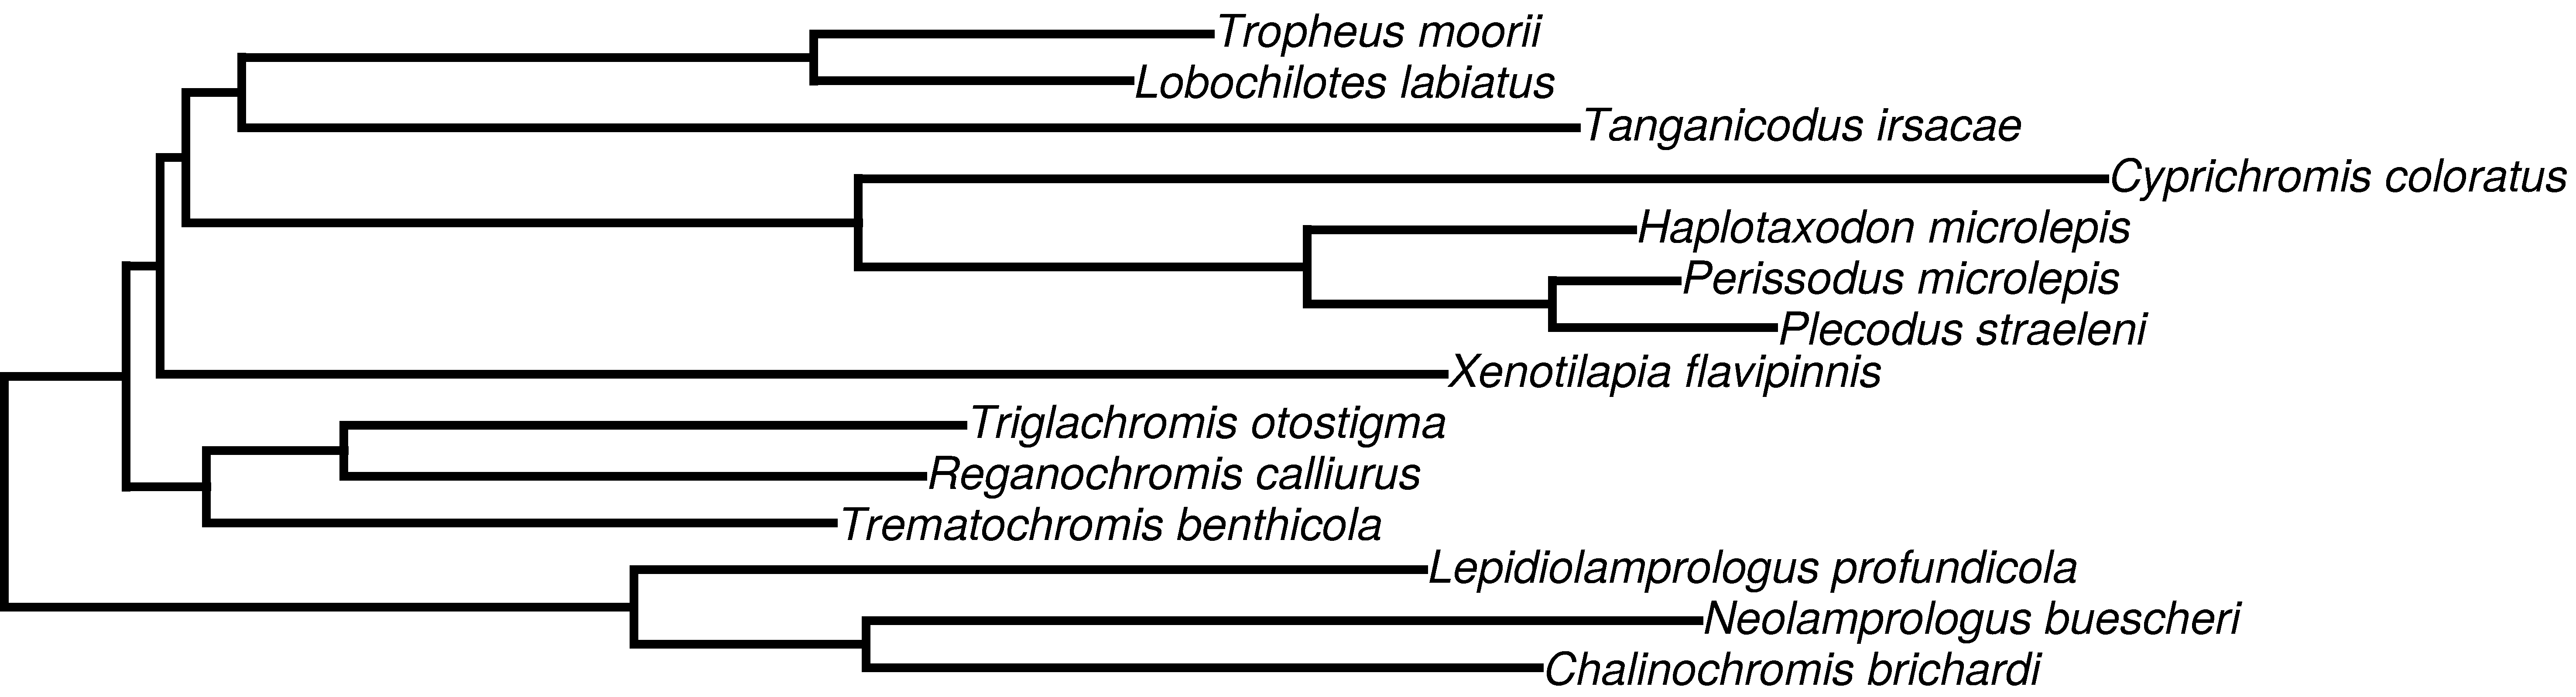
\includegraphics[width=\textwidth]{FishPoo/figures/mcgee_tree.pdf}
%    \caption{A maximum likelihood phylogeny of the host organisms.}
%    \label{FP_host_tree}
%\end{figure}

\subfile{FishPoo/figures/figure2}

\subsection{Sample collection}

After shipping, specimens were placed in tanks separated by species. Where only one member of a species was collected, they were placed in a solitary tank. Specimens were allowed to acclimatize to their tanks and observed for signs of injury or stress. Because fish are usually starved prior to shipping to prevent stool decomposition from suffocating them in transit, feeding began as soon as it deemed safe. All specimens were fed a common diet of kelp and \textit{Arthrospira platensis} pellets (Omega One brand Veggie Mini Pellets) for six weeks. 

For sample collection, specimens were fed until satiated and placed into 30L tanks. To minimize microbial contamination in the water and tank silicone, we lined each tank with a sterile autoclave bag prepared with 10 liters of molecular water augmented with a 5 grams each of sodium chloride and calcium chloride. To minimize potential contamination from biological filtration, we used chemical filtration via sterile charcoal pellets (Petco brand activated carbon pellets boiled in molecular water for 20 minutes) to sequester nitrogenous wastes produced by the fish, and a vinyl aquarium tube was submerged and connected to an air pump to aerate the water. For each collection, fresh tubing was flushed and wiped down with ethanol and dried before use. After feeding, specimens were transferred into the collection tanks and checked frequently until stool was observed. If no stool was observed within 24 hours, the specimen was returned to a standard vivarium tank and the experiment was repeated. After removing the specimen from the collection tank, stool was removed using a sterile serological pipette and frozen. 

\subsection{Sample preparation, processing and sequencing}

Stool samples were subjected to bead beating for 60 seconds and DNA was extracted using MoBio PowerSoil DNA Isolation kit in accordance with the manufacturer's protocol. DNA yields were measured using a Qubit Fluorometer (Invitrogen) and Quant-iT dsDNA Assay Kit, High Sensitivity (Invitrogen product no. Q33120). DNA was amplified by a two-step PCR enrichment of the V4 region of the 16S rRNA gene using ``universal'' primers 515F (TGCCAGCMGCCGCGGTAA) and 806R (GGACTACHVGGGTWTCTAAT), modified by addition of Illumina adapter and barcodes sequences (See Table \ref{FP_barcodes}).

\subfile{FishPoo/tables/table3}

\begin{table}[]
\centering
\caption{PCR cycling conditions}
\label{my-label}
\begin{tabular}{@{}ll@{}}
\toprule
Temperature (\degree C) & Time (mm:ss)       \\ \midrule
95\degree C             & 2:00               \\ \midrule
95\degree C             & 0:15               \\
52\degree C             & 0:30               \\
72\degree C             & 1:30               \\
Repeat                  & $\times 10$ cycles \\ \midrule
72\degree C             & 3:00               \\
4\degree C              & Forever            \\ \bottomrule
\end{tabular}
\end{table}

PCR products were then purified using magnetic bead capture of high molecular weight DNA (Agricourt Ampure XP beads; product number A63880).

Libraries were sequenced using an Illumina MiSeq system, generating 250 base pair paired-end amplicon reads. The amplicon data was multiplexed using dual barcode combinations for each sample. A custom script available in a GitHub repository (\url{https://github.com/gjospin/scripts/blob/master/Demul_trim_prep.pl}), to assign each pair of reads to their respective samples when parsing the raw data. This script allows for one base pair difference per barcode. The paired reads were then aligned and a consensus was computed using {\tt Trimmomatic} \cite{bolger2014trimmomatic} with maximum overlap of 120 and a minimum overlap of 70 (other parameters were left as default). The custom script automatically demultiplexes the data into {\tt fastq} files and parses the results to reformat the sequences in {\tt fasta} format.

\subsection{Building the observation table}

Chimera were identified with {\tt vsearch}, \cite{rognes2016vsearch} and unique reads were identified using {\tt hat-trie}. \cite{askitis2005cache, askitis2007hat} A table of observation counts were constructed as a {\tt Pandas} {\tt DataFrame} object, \cite{mckinney2010data} and a count threshold was applied. Tables of raw counts and normalized counts were written as comma separated value files, and the corresponding sequences were written as a FASTA file. All analysis was carried out and documented in Jupyter Notebooks \cite{perez2007ipython} and visualizations, including all those appearing in this manuscript, were constructed using {\tt Matplotlib}. \cite{hunter2007matplotlib}

\subsection{Building phylogeny of OTUs}

The Illumina sequencing platform has a substitution error frequency of about 0.1\%. \cite{ross2013characterizing} Trimming and filtering reads based on quality score removes about 69\% of substitution errors, on average, \cite{schirmer2016illumina} and overlap correcting paired-end reads improves this to about one substitution error in every 14 reads. \cite{bolger2014trimmomatic} At the sacrifice of sensitivity, the error frequency can be reduced arbitrarily by excluding very rare sequences. For example, excluding sequences observed only once reduces the substitution error frequency to about one in every 200 sequences. Most substitution errors are likely to be corruptions of sequences already present in the data, and so phylogenetic reconstruction should place them as sister leafs of their uncorrupted sources. This confines the effect of substitution errors to the smallest topological scale, where it appears in the form of ``extra'' leafs that are randomly attached with the minimum branch length.

Alignment of the observed sequences is performed using {\tt Clustal Omega}, \cite{goujon2010new, sievers2011fast} and an approximate maximum likelihood phylogeny is constructed using {\tt FastTree}. \cite{price2009fasttree, price2010fasttree}

%\begin{figure}
%    \includegraphics[width=\textwidth]{FishPoo/figures/fishpoo_tree.png}
%    \caption{An approximate maximum likelihood phylogeny of the guest organisms.}
%    \label{FP_guest_tree}
%\end{figure}

\subfile{FishPoo/figures/figure3}

\subsection{Spectral analysis and machine learning}

%In phylogeographic models, network edges edges represent dispersal rates, a convolution of both the vectors of dispersal and the barriers that impinge on those vectors. Organisms move from habitat to habitat in discrete events with probabilities related to the dispersal rates. If organisms are gathered from each habitat, and trees of related organisms are constructed, these trees may be used to infer the rates of dispersal. These rates reveal, at least in broad strokes, the structure of the relationships among the habitats.

The host tree and guest tree are loaded as {\tt SuchTree} objects, and linked together through the observation table as a {\tt SuchLinkedTrees} object. The {\tt SuchTree} class allows for extremely efficient traversals of large trees, enabling distance correlations to be efficiently computed. The {\tt SuchLinkedTrees} class leverages this to compute graph adjacency and graph Laplacian matrixes of subtrees of host and guest phylogenies. Spectral decomposition and kernel densities of graph Laplacians are computed using {\tt numpy}, and the Jensen-Shannon divergence is calculated between each pair of spectral densities using the {\tt entropy} function in {\tt scipy.stats}. \cite{walt2011numpy} Feature tables were assembled using {\tt Pandas} \cite{mckinney2010data} and machine learning was carried out using {\tt scikit-learn}. \cite{pedregosa2011scikit}

\subsection{Correlation-based analysis}

For each clade of guest organisms, the {\tt SuchLinkedTrees.linked\_distances} function is used to calculate the pairwise distances through the host and guest trees for every pair of non-null observations in the link matrix, as described by Hommola {\em et al.} \cite{hommola2009permutation} The Pierson's correlation for these distances is computed using the {\tt pearsonr} function from {\tt scipy.stats}. \cite{walt2011numpy}

\subsection{Literature search for comparative analysis}

Trees and interaction matrixes were compiled from the supplementary material from Rezende {\em et al.}, \cite{rezende2007non} Hafner {\em et al.} \cite{hafner1994disparate} and Escudero \cite{escudero2015phylogenetic} for a total of fifty data sets (Table \ref{FP_studies_table}). Taxonimic identifiers were reconciled between trees and interaction matrixes using Levenshtein distances \cite{levenshtein1966binary} calculated using {\tt fuzzywuzzy}, \cite{fuzzywuzzy} and by hand where necessary. Corrected trees and matrixes are distributed with permission with {\tt SuchTree} in Newick format and comma separated values, respectively.

\subsection{Simulated datasets}

Synthetic interactions with perfect phylogenetic congruence and with no phylogenetic congruence were simulated using {\tt Dendropy}. \cite{sukumaran2010dendropy} The birth and death rates of trees from the literature was estimated with the gamma statistic \cite{pybus2000testing} using {\tt Dendropy}, and random trees were generated so that the distribution of the number of taxa and their birth and death rates would match the trees from the literature. Two sets of random interactions were generated; a set of `perfect' interactions, where the tips of two identical random trees were linked by a simple bijection, and a set of `null' interactions, where the tips of to independently generated random trees were linked with a random shuffle. The set of `perfect' interactions simulates a coevolutionary process in which the evolution of the interacting groups proceeds in lockstep. The `null' interactions simulate a small subset of possible ecological interactions in which no coevolution has taken place.